\chapter{Analysis}

\section{Introduction}

\subsection{Client Identification}
My client's name is Lee Travers. He is 45 years old and has almost no experience with computers other than a few very basic tasks. He mainly uses his computer to occasionally send emails. Currently, Lee uses manual paper methods to oversee current items in stock and to control the stock and he uses his HP laptop running Windows 10 to send emails.

Lee is a self employed plumber, who runs a Fishing tackle shop on the side. In his shop he sells many products such as fishing rods, bait, fishings reels, line and other necessities for a fishing trip. His shop is located in Sawston and he gets shipments of stock from many big brands. Lee usually runs the shop alone, however he often has assistance from his brother in law or his father in law when he is unable to be in the shop, due to his other job.

Lee would like to use an ICT based system in order to boost the business's productivity and speed of work. Currently, with the paper based system, he finds it difficult to keep track of which items are in stock and how many there are, and keeping all the data in one place. With the new system, Lee would like to keep the stock control in a database, so he can easily edit which items are available and to keep all the data centralized.

\subsection{Define the current system}
The current system in use is a manual paper based system. Lee uses a book and writes down what products are currently in stock and how many of each product are left. Eventually this gets quite messy, due to having to cross out numbers and write in new ones. The book mainly contains information on current stocks, stocks that are reserved for a particular customer and orders that need to be made.

When it is necessary for Lee to make an order, he notes down the stock that has run out and contacts his supplier and makes an order. When the stock arrives, he adds the product and amount to the book.

\subsection{Describe the problems}
There are many problems with this system. First, the book gets incredibly messy very quickly, because of crossing out numbers etc. The book also fills up very quickly, since the shop sells out quite fast, and new orders and new stock have to be added in, so the book is replaced often. Also, due to the messiness of the book, it is very difficult to keep track of the items that are actually in stock, so he often doesn't know which products he needs to order. 

\subsection{Section appendix}

\section{Investigation}

\subsection{The current system}

\subsubsection{Data sources and destinations}
In the current system, there are t hree data sources that are used, the product, the customer and the supplier. Product tells which products are currently in stock and how much they are being sold for each item. Customer is used when a customer makes a reservation for a product. It tells the details of the customer and which products and how many they want. Supplier is used when stock is running out and has to be replaced. It tells the name of the supplier, the product name, the quantity and price.

\begin{center}
\begin{tabular}{| l | p{5cm} | l | l |}
    \hline
    \textbf{Source} & \textbf{Data} & \textbf{Example Data} & \textbf{Destination} \\ \hline
    Product & Product Name, Price, Quantity & Fishing Rod, £99.99, 10 & Owner \\ \hline
    Customer & Customer Name,, Telephone No., Product Name, Quanitity & John Smith, 12345678910 & Owner \\ \hline
    Supplier & Supplier Name, Product Name, Quantity, Price & Nash, Rod, 4, £99.99 & Owner \\ \hline
  
\end{tabular}
\label{tab:range_examples}
\end{center}

\subsubsection{Algorithms}
In the current system there are three algorithms in use. One is checking if a product is in stock. Another is making reservations of products for a customer. Another is ordering a product if it is out of stock.


\begin{algorithm}[H]
    \caption{Checking if a product is in stock}
\begin{algorithmic}[1]
\SET{$available$}{$false$}
\State
\While{$not available$}
    \SEND{$"Please\ choose\ a\ product\ (0 to finish)"$}
    \RECEIVE{$product$}
    \If{$Product > 0$}
        \SET{$available$}{$true$}
    \EndIf
\EndWhile
\end{algorithmic}
\end{algorithm}


\begin{algorithm}[H]
    \caption{Making reservations}
\begin{algorithmic}[2]
\SET{$order$}{$false$}
\State
\While{$not order$}
    \SEND{$"Please\ choose\ a\ product\ (0 to finish)"$}
    \RECEIVE{$product$}
    \If{$Product > 0$}
        \SET{$order$}{$true$}
    \EndIf
\EndWhile
\end{algorithmic}
\end{algorithm}

\begin{algorithm}[H]
    \caption{Ordering in new stock}
\begin{algorithmic}[3]
\SET{$available$}{$false$}
\State
\While{$not available$}
    \SEND{$"Please\ choose\ a\ product\ (0 to finish)"$}
    \RECEIVE{$product$}
    \If{$Product < 0$}
        \SET{$available$}{$true$}
        the product is ordered
    \EndIf
\EndWhile
\end{algorithmic}
\end{algorithm}

\subsubsection{Data flow diagram}

\begin{figure}[H]
	\centering
	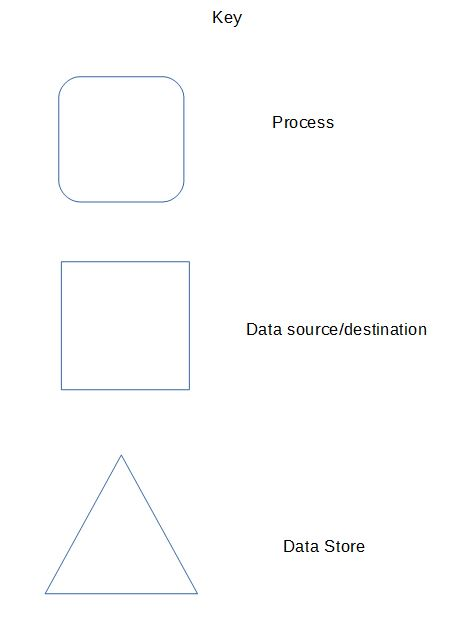
\includegraphics[width= 10cm, height = 15.5cm]{Analysis/images/dfd_key.JPG}
	\caption {Data Flow Diagram Key} \label{fig:data_diagram_key}
\end{figure}

\begin{figure}[H]
	\centering
	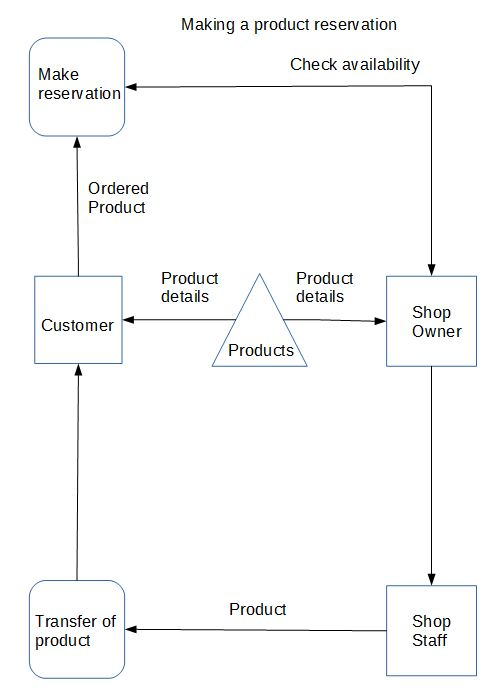
\includegraphics[width= 10cm, height = 15.5cm]{Analysis/images/reserving_dfd.JPG}
	\caption {Reserving a Product Data Flow Diagram} \label{fig:reserving_data_diagram}
\end{figure}

\begin{figure}[H]
	\centering
	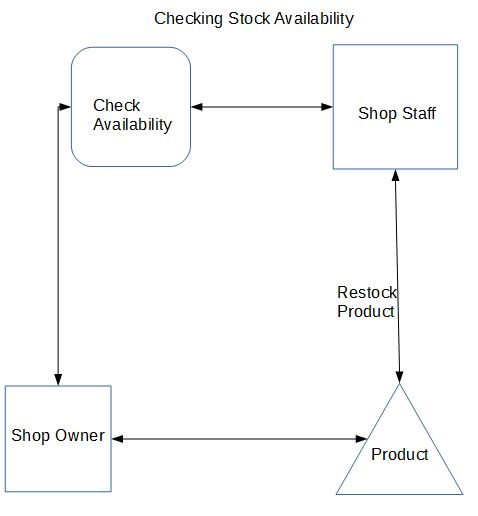
\includegraphics[width= 10cm, height = 12cm]{Analysis/images/stock_check_dfd.JPG}
	\caption {Checking Availability of Stock Data Flow Diagram} \label{fig:checking_stock_data_diagram}
\end{figure}

\begin{figure}[H]
	\centering
	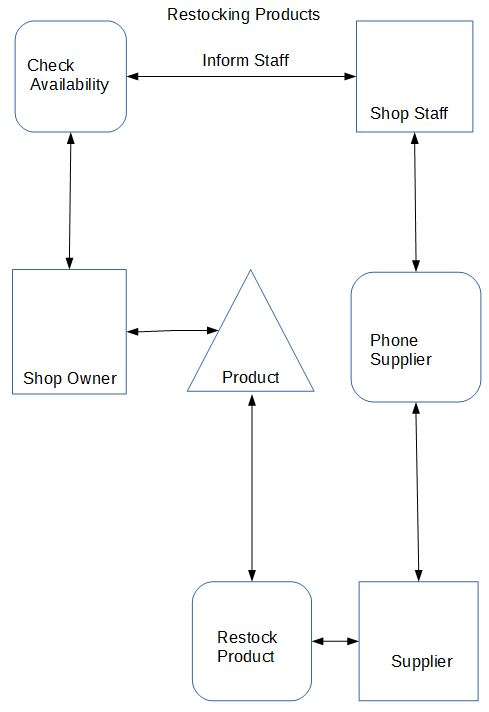
\includegraphics[width= 10cm, height = 15.5cm]{Analysis/images/restock_dfd.JPG}
	\caption {Restocking Products Data Flow Diagram} \label{fig:restocking_data_diagram}
\end{figure}
\subsubsection{Input Forms, Output Forms, Report Formats}

\subsection{The proposed system}

\subsubsection{Data sources and destinations}
\begin{figure}[H]
	\centering
	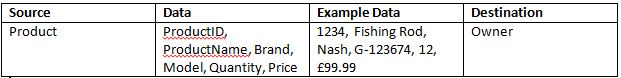
\includegraphics[width= 15cm, height = 2cm]{Analysis/images/data_sources.JPG}
	\caption {Data Sources and Destinations} \label{fig:data_sources}
\end{figure}
\subsubsection{Data flow diagram}

\subsubsection{Data dictionary}
\begin{figure}[H]
	\centering
	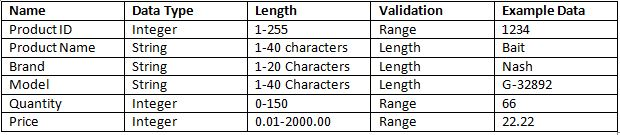
\includegraphics[width= 15cm, height = 4cm]{Analysis/images/data_dictionary.JPG}
	\caption {Data Dictionary} \label{fig:data_dictionary}
\end{figure}

\subsubsection{Volumetrics}
The System should be able to to up to 500 different products. I chose this number as the shop stores around 100 different products, with different models and brands, so 500 is a good amount for this.
\section{Objectives}

\subsection{General Objectives}
\begin{itemize}
	\item Clear/ easy to understand layout structure for Product Record viewing
	\item Clear/ easy to understand layout structure for Product data input
\end{itemize}
\subsection{Specific Objectives}
Product Record Viewing
\begin{itemize}
	\item Clear set out labels for each attribute of data.
	\item Minimal controls to keep the viewing of records basic and easily accessible
\end{itemize}
Product Data Input
\begin{itemize}
	\item Simple input boxes clearly labelled for each attribute
	\item Drop down boxes for attributes such as quantity
\end{itemize}
\subsection{Core Objectives}
\begin{itemize}
	\item Product Records viewing
	\item Product Data Input
\end{itemize}
\subsection{Other Objectives}
\begin{itemize}
	\item Ordering New Products
	\item Reserving Products
\end{itemize}
\section{ER Diagrams and Descriptions}

\subsection{ER Diagram}

\subsection{Entity Descriptions}

\section{Object Analysis}

\subsection{Object Listing}

\subsection{Relationship diagrams}

\subsection{Class definitions}

\section{Other Abstractions and Graphs}

\section{Constraints}

\subsection{Hardware}

\subsection{Software}

\subsection{Time}

\subsection{User Knowledge}

\subsection{Access restrictions}

\section{Limitations}

\subsection{Areas which will not be included in computerisation}

\subsection{Areas considered for future computerisation}

\section{Solutions}

\subsection{Alternative solutions}

\subsection{Justification of chosen solution}